% vim: set textwidth=78 autoindent:

% \subsection{GPS Plugin}\label{label_plugingps}
\subsection{Plugin GPS}\label{label_plugingps}

% when the revision of a section has been finalized,
% comment out the following line:
% \updatedisclaimer

% \subsubsection{What is GPS?}\label{whatsgps}
\subsubsection{Qu'est ce qu'un GPS ?}\label{whatsgps}

% GPS, the Global Positioning System, is a satellite-based system that allows 
% anyone with a GPS receiver to find their exact position anywhere in the world.
% It is used as an aid in navigation, for example in airplanes, in boats and by 
% hikers.
Le GPS, Global Positioning System, est un syst\`eme bas\'e sur des satellites qui
permet \`a toute personne poss\'edant un r\'ecepteur GPS d'obtenir sa position exacte
n'importe o\`u dans le monde. Il est utilis\'e comme aide \`a la navigation, comme par
exemple pour les avions, dans les bateaux et par les voyageurs.
% The GPS receiver uses the signals from the satellites to calculate its
% latitude, longitude and (sometimes) elevation.
Le r\'ecepteur GPS utilise les signaux des satellites pour calculer la latitude,
la longitude et (parfois) l'\'el\'evation.
% Most receivers also have the capability to store locations (known as 
% \emph{waypoints}), sequences of locations that make up a planned \emph{route}
% and a tracklog or \emph{track} of the receivers movement over time.
La plupart des r\'ecepteurs ont \'egalement la possibilit\'e de stocker la position
(nomm\'e \emph{waypoints}), des s\'equences de positions qui constituent un
\emph{itin\'eraire} pr\'evu et un tracklog ou \emph{track} des d\'eplacements du
r\'ecepteur en fonction du temps.
% Waypoints, routes and tracks are the three basic feature types in GPS data.
% QGIS displays waypoints in point layers while routes and tracks are displayed
% in linestring layers.
Waypoints, itin\'eraires et tracks sont les trois types d'objet basic dans les
donn\'ees GPS. QGIs affiche les waypoints dans des couches points tandis que les
itin\'eraires et les tracks sont affich\'es dans des couches lin\'eaires.

% \subsubsection{Loading GPS data from a file}\label{label_loadgps}
\subsubsection{Charger des donn\'ees GPS \`a partir d'un
fichier}\label{label_loadgps}

% There are dozens of different file formats for storing GPS data.
Il y a des dizaines de formats de fichier diff\'erent pour stocker des donn\'ees
GPS.
% The format that QGIS uses is called GPX (GPS eXchange format), which is a 
% standard interchange format that can contain any number of waypoints, routes
% and tracks in the same file.
Le format que QGIS utilise est appel\'e GPX (GPS eXchange format), qui est un
format d'\'echange standard qui peut contenir n'importe quel nombre de waypoints,
itin\'eraire et tracks dans un m\^eme fichier.

% To load a GPX file you first need to load the plugin \mainmenuopt{Plugins} >
% \dropmenuopttwo{mActionShowPluginManager}{Plugin Manager...} > \checkbox{GPS
% Tools}. When this plugin is loaded a button with a small handheld GPS device
% will show up in the toolbar. An example GPX file is available in the QGIS
% sample dataset: \filename{/qgis\_sample\_data/gps/national\_monuments.gpx}.
% See Section~\ref{label_sampledata} for more information about the sample data.
Pour charger un fichier GPX vous devez d'abord charger le plugin
\mainmenuopt{Plugins} > \dropmenuopttwo{mActionShowPluginManager}{Gestionnaire
de Plugin} > \checkbox{Outils GPS}. Quand cette extension est charg\'ee, un bouton avec
un petit p\'eriph\'erique GPS appara\^itra dans la barre d'outils. Un fichier GPX
d'exemple est disponible dans le jeu de donn\'ees d'exemple de QGIS :
\filename{/qgis\_sample\_data/gps/national\_monuments.gpx}. Voir 
Section~\ref{label_sampledata} pour plus d'information sur les donn\'ees
d'exemple.

\begin{enumerate}
% \item Click on the \toolbtntwo{gps_importer}{GPS Tools} icon and open the
% \tab{Load GPX file} tab.
\item cliquez sur l'ic\^one \toolbtntwo{gps_importer}{Outils GPS} et ouvrez 
l'onglet \tab{Charger un fichier GPX}
% \item \button{Browse} to the folder \filename{qgis\_sample\_data/gps/},
% select the GPX file \filename{national\_monuments.gpx} and click
% \button{Open}.
\item \button{Naviguez} vers le r\'epertoire \filename{qgis\_sample\_data/gps/},
s\'electionnez le fichier GPX \filename{national\_monuments.gpx} et cliquez sur le
bouton \button{Ouvrir}.
\end{enumerate}

\begin{figure}[ht]
   \begin{center}
% \caption{\label{gpxloader}The \emph{GPS Tools} dialog window \nixcaption}
\caption{\label{gpxloader}La bo\^ite de dialogue de l'\emph{Outils
GPS}\nixcaption}
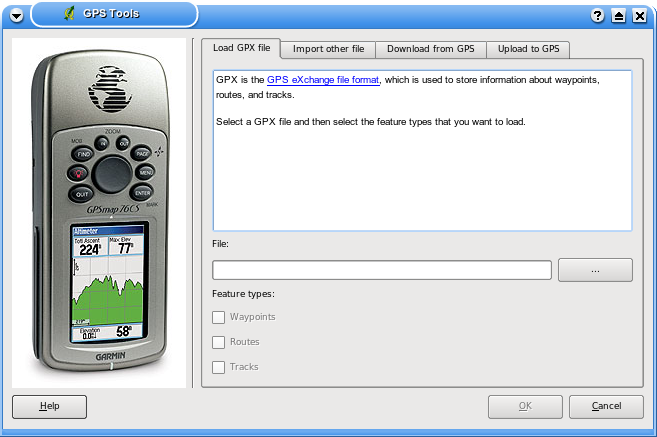
\includegraphics[clip=true, width=12cm]{loadgpx}
\end{center}
\end{figure}

% Use the browse button \browsebutton to select the GPX file, then use the
% checkboxes to select the feature types you want to load from that GPX file.
% Each feature type will be loaded in a separate layer when you click
% \button{OK}. The file \filename{national\_monuments.gpx} only includes
% waypoints.
Utilisez le bouton \browsebutton pour s\'electionner le fichier GPX, puis
utilisez la case \`a cocher pour s\'electionner les types de g\'eom\'etrie que vous
voulez charger \`a partir de ce fichier GPX. Chaque type d'objet sera charg\'e
dans une couche s\'epar\'ee lors du clique sur le bouton \button{OK}. Le fichier 
\filename{national\_monuments.gpx} inclue seulement des waypoints.

% \subsubsection{GPSBabel}
\subsubsection{GPSBabel}

% Since QGIS uses GPX files you need a way to convert other GPS file formats to
% GPX. This can be done for many formats using the free program GPSBabel, which
% is available at \url{http://www.gpsbabel.org}.
Puisque QGIs utilise des fichiers GPX vous avez besoin de convertir les autres
formats de fichiers GPS en GPX. Cela peut \^etre r\'ealis\'e pour plusieurs formats
en utilisant le logiciel libre GPSBabel qui est disponible sur
\url{http://www.gpsbabel.org}.
% This program can also transfer GPS data between your computer and a GPS
% device. QGIS uses GPSBabel to do these things, so it is recommended that you
% install it. However, if you just want to load GPS data from GPX files you will
% not need it. Version 1.2.3 of GPSBabel is known to work with QGIS, but you
% should be able to use later versions without any problems.
Ce programme peut aussi transf\'erer des donn\'ees GPS entre votre ordinateur et
un p\'eriph\'erique GPS. QGIS utilise GPSBabel pour r\'ealiser ces t\^aches, il est
donc recommand\'e de l'installer. Cependant si vous voulez juste charger des
donn\'ees \`a partir de fichiers GPX vous n'en avez pa besoin. La version 1.2.3 de
GPSBabel est connue pour bien fonctionner avec QGIS, mais vous pouvez
devriez pouvoir utiliser des versions plus r\'ecentes sans probl\`eme.

% \subsubsection{Importing GPS data}
\subsubsection{Importer des donn\'ees GPS}

% To import GPS data from a file that is not a GPX file, you use the tool 
% \tab{Import other file} in the GPS Tools dialog. Here you select the file that
% you want to import, which feature type you want to import from it, where you
% want to store the converted GPX file and what the name of the new layer should
% be.
Pour importer des donn\'ees d'un fichier qui n'est pas un fichier GPX, vous devez
utiliser l'outil \tab{Importer d'autres fichiers} dans la bo\^ite de dialogue des
outils GPS. Vous s\'electionnez le fichier que vous voulez importer, quel type de
g\'eom\'etrie vous voulez importer de ce celui-ci, o\`u vous voulez stocker le
fichier GPX converti et sous quel nom enregistrer la couche.

% When you select the file to import you must also select the format of that
% file by using the menu in the file selection dialog (see figure \ref{figure
% importdialog}). All formats do not support all three feature types, so for
% many formats you will only be able to choose between one or two types.
Quand vous s\'electionnez le fichier \`a importer vous devez \'egalement s\'electionner
le format de ce fichier en utilisant le menu dans la bo\^ite de dialogue de
s\'election de fichiers (voir la figure~\ref{figure_importdialog}). Tous les
formats ne g\`erent pas les 3 types de g\'eom\'etries, vous pourrez donc choisir pour
plusieurs formats qu'un ou deux types.

\begin{figure}[ht]
   \begin{center}
% \caption{\label{figure importdialog}File selection dialog for the import
% tool \nixcaption}
\caption{\label{figure_importdialog}Bo\^ite de dialogue de s\'election de fichier
pour l'outil import\nixcaption}
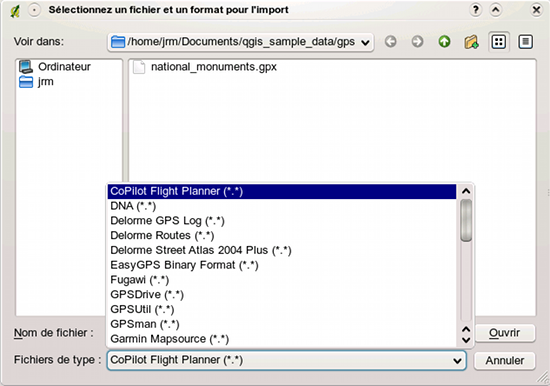
\includegraphics[clip=true, width=12cm]{importdialog}
   \end{center}
\end{figure}

% \subsubsection{Downloading GPS data from a device}
\subsubsection{T\'el\'echarger des donn\'ees GPS \`a partir d'un p\'eriph\'erique}

% QGIS can use GPSBabel to download data from a GPS device directly into vector 
% layers.
QGIS peut utiliser GPSBabel pour t\'el\'echarger des donn\'ees d'un p\'eriph\'erique GPS
directement dans des couches vecteurs.
% For this you use the tool \tab{Download from GPS} (see Figure
% \ref{figure_download}), where you select your type of GPS device, the port
% that it is connected to, the feature type that you want to download, the GPX
% file where the data should be stored, and the name of the new layer.
Pour cela, utilisez l'outil \tab{T\'el\'echarger d'un GPS} (voyez la
figure~\ref{figure_download}), o\`u vous choisissez votr etype de p\'eriph\'erique
GPS, le port auquel il est connect\'e, le type de g\'eom\'etrie que vous voulez
t\'el\'echarger, le fichier GPX o\`u les donn\'ees doivent \^etre stock\'ees et le nom de la
nouvelle couche.

\begin{figure}[ht]
   \begin{center}
% \caption{\label{figure_download}The download tool \nixcaption}
\caption{\label{figure_download}L'outil de t\'el\'echargement\nixcaption}
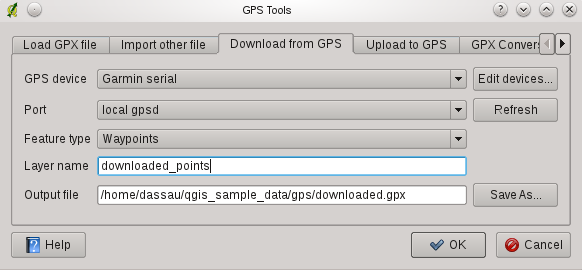
\includegraphics[clip=true, width=12cm]{download}
   \end{center}
\end{figure}

% The device type you select in the GPS device menu determines how GPSBabel
% tries to communicate with the device.
Le type de p\'eriph\'erique que vous s\'electionner dans le menu p\'eriph\'erique GPS
d\'etermine comme GPSBabel tente de communiquer avec votre p\'eriph\'erique.
% If none of the types works with your GPS device you can create a new type
% (see section \ref{sec:Defining-new-device}).
Si aucun des types ne fonctionne avec votre p\'eriph\'erique GPS, vous pouvez cr\'eer
un nouveau type adapt\'e (voir la section \ref{sec:Defining-new-device}).

% The port is a file name or some other name that your operating system uses as
% a reference to the physical port in your computer that the GPS device is
% connected to.
Le port est un nom de fichier ou autre nom que votre syst\`eme d'op\'eration
utilise comme une r\'ef\'erence du port physique de votre ordinateur auquel le
p\'eriph\'erique GPS est connect\'e.
% \nix On Linux this is something like /dev/ttyS0 or /dev/ttyS1 and on \win 
% Windows it's COM1 or COM2.
\nix Sous Linux cela ressemble \`a /dev/ttyS0 ou /dev/ttyS1  et sous \win 
Windows c'est COM1 ou COM2.

% When you click \button{OK} the data will be downloaded from the device and 
% appear as a layer in QGIS.
Quand vous cliquez sur le bouton \button{OK} les donn\'ees seront t\'el\'echarg\'ees du
p\'eriph\'erique et appara\^itront dans une couche dans QGIS.

\subsubsection{Uploading GPS data to a device}

% You can also upload data directly from a vector layer in QGIS to a GPS device, 
% using the tool \tab{Upload to GPS}.
Vous pouvez \'egalement envoyer directement vos donn\'ees d'une couche vecteur 
dans QGIS vers un p\'eriph\'erique GPS en utilisant l'outil \tab{Upload to GPS}.
% The layer must be a GPX layer.
La couche doit \^etre une couche GPX.
% To do this you simply select the layer that you want to upload, the type of 
% your GPS device and the port that it's connected to.
Pour r\'ealiser cela, vous s\'electionnez simplement la couche que vous voulez 
uploader, le type de votre p\'eriph\'erique GPS et le port auquel il est connect\'e.
% Just as with the download tool you can specify new device types if your device 
% isn't in the list.
De la m\^eme mani\`ere que pour l'outil de t\'el\'echargement, vous pouvez d\'efinir de 
nouveaux types de p\'eriph\'erique si le v\^otre n'est pas dans la liste.

% This tool is very useful together with the vector editing capabilities of QGIS.
% You can load a map, create some waypoints and routes and then upload them and 
% use them in your GPS device.
Cet outil est tr\`es utile avec les possibilit\'es d'\'edition vectorielle de QGIS. 
Vous pouvez charger une carte, cr\'eer des waypoints et des routes puis les
t\'el\'echarger et les utiliser dans votre p\'eriph\'erique QGPS.

% \subsubsection{\label{sec:Defining-new-device}Defining new device types}
\subsubsection{\label{sec:Defining-new-device}D\'efinir de nouveaux types de p\'e
riph\'eriques}

% There are lots of different types of GPS devices.
Il y a beaucoup de types diff\'erents de p\'eriph\'eriques GPS.
% The QGIS developers can't test all of them, so if you have one that does not 
% work with any of the device types listed in the \tab{Download from GPS} and
% \tab{Upload to GPS} tools you can define your own device type for it.
Les d\'eveloppeurs de QGIS ne peuvent pas les tester tous, si vous en avez un qui
ne fonnctione pas avec un des types de p\'eriph\'eriques dans les outils
\tab{R\'ecup\'erer du GPS} et \tab{T\'el\'echarger du GPS}, vous pouvez d\'efinir votre
propre type de p\'eriph\'erique.
% You do this by using the GPS device editor, which you start by clicking the 
% \button{Edit devices} button in the download or the upload window.
Vous r\'ealisez cela en utilisant l'\'editeur de p\'eriph\'erique de GPS, que vous
d\'emarrez en cliquant le bouton \button{\'Editer un p\'eriph\'erique} dans la fen\^etre
de r\'ecup\'eration ou de t\'el\'echargement.

% To define a new device you simply click the \button{New device} button, enter
% a name, a download command and an upload command for your device, and click
% the \button{Update device} button.
Pour d\'efinir un nouveau p\'eriph\'erique, vous cliquez sur le boutton
\button{Nouveau p\'eriph\'erique}, entrez un nom, une commande de r\'ecup\'eration et
une commande de t\'el\'echargement pour votre p\'eriph\'erique, et cliquez sur le
bouton \button{Mise \`a jour du p\'eriph\'erique}.
% The name will be listed in the device menus in the upload and download
% windows, and can be any string.
Le nom sera list\'e dans les menus des p\'eriph\'eriques dans la fen\^etre r\'ecup\'eration
et t\'el\'echargement, et peut \^etre n'importe quelle cha\^ine de caract\`ere.
% The download command is the command that is used to download data from the 
% device to a GPX file.
La commande de r\'ecup\'eration est la commande qui est utilis\'ee pour r\'ecup\'erer les
donn\'ees du p\'eriph\'erique vers un fichier GPX.
% This will probably be a GPSBabel command, but you can use any other command 
% line program that can create a GPX file.
Ce sera certainement une commande GPSBabel, mais vous pouvez utiliser un autre
programme en ligne de commande qui cr\'e\'e un fichier GPX.
% QGIS will replace the keywords \usertext{\%type}, \usertext{\%in}, and 
% \usertext{\%out} when it runs the command.
QGIS remplacera les mots-cl\'e \usertext{\%type}, \usertext{\%in}, et
\usertext{\%out} lorsqu'il lancera la commande.

% \usertext{\%type} will be replaced by {}``\usertext{-w}'' if you are 
% downloading waypoints, {}``\usertext{-r}'' if you are downloading routes and
% {}``\usertext{-t}'' if you are downloading tracks.
\usertext{\%type} sera remplac\'e par {}``\usertext{-w}''  si vous t\'el\'echargez
des waypoints, {}``\usertext{-r}'' si vous t\'el\'echargez des routes et
{}``\usertext{-t}'' si vous t\'el\'echargez des tracks.
% These are command line options that tell GPSBabel which feature type to
% download.
Ce sont des options de la ligne de commande qui dit \`a GPSBabel quel type
d'objet  \`a t\'el\'echarger.

% \usertext{\%in} will be replaced by the port name that you choose in the 
% download window and \usertext{\%out} will be replaced by the name you choose 
% for the GPX file that the downloaded data should be stored in.
\usertext{\%in} sera remplac\'e par le port que vous avez choisi dans la bo\^ite de
dialogue de t\'el\'echargement et \usertext{\%out} sera remplac\'e par le nom que
vous avez choisi pour le fichier GPX o\`u les donn\'ees t\'el\'echarg\'ees doivent \^etre
stock\'ees.
% So if you create a device type with the download command
% {}``\usertext{gpsbabel\%type -i garmin -o gpx \%in \%out}'' (this is actually
% the download command for the predefined device type \selectstring{GPS
% device:}{Garmin serial})and then use it to download waypoints from port
% {}``\usertext{/dev/ttyS0}'' to the file {}``\usertext{output.gpx}'', QGIS will
% replace the keywords and run the command {}``\usertext{gpsbabel -w -i garmin
% -o gpx /dev/ttyS0 output.gpx}''.
Si vous cr\'eez un type de p\'eriph\'erique avec la commande de t\'el\'echargement
{}``\usertext{gpsbabel\%type -i garmin -o gpx \%in \%out}'' (c'est actuellement
la commande de t\'el\'echargement pour le type de p\'eriph\'erique pr\'ed\'efini
\selectstring{GPS device:}{Garmin serial}) puis utilisez-le pour t\'el\'echarger
les waypoints \`a partir du port {}``\usertext{/dev/ttyS0}''  vers le fichier
{}``\usertext{output.gpx}'', QGIS remplacera les mots-cl\'es et lancera la
commande {}``\usertext{gpsbabel -w -i garmin -o gpx /dev/ttyS0 output.gpx}''.

% The upload command is the command that is used to upload data to the device.
% The same keywords are used, but \usertext{\%in} is now replaced by the name of 
% the GPX file for the layer that is being uploaded, and \usertext{\%out} is
% replaced by the port name.
La commande de t\'el\'echargement est la commande qui est utilis\'ee pour t\'el\'echarger 
des donn\'ees vers le p\'eriph\'erique. Le m\^eme mot-cl\'e est utilis\'e, mais 
\usertext{\%in} est maintenant remplac\'e par le nom du fichier GPX pour la couche
qui est en t\'el\'echarg\'ee et \usertext{\%out} est remplac\'e par le nom du port.

% You can learn more about GPSBabel and it's available command line options at 
% \url{http://www.gpsbabel.org}
Vous pouvez en savoir plus sur GPSBabel et ses options de ligne de commande
disponible sur \url{http://www.gpsbabel.org}.

% Once you have created a new device type it will appear in the device lists
% for the download and upload tools.
Une fois le nouveau type de p\'eriph\'erique cr\'e\'e celui-ci apparaitra dans les
listes de p\'eriph\'erique dans les outils de r\'ecup\'eration et de t\'el\'echargement.

